\documentclass[noback]{cuposter}

%%\documentclass[noback,portrait]{cuposter}
%% To make a poster in portrait, use the "portrait" option to
%% documentclass as shown above.
\usepackage{caption}
\usepackage{enumitem}
\usepackage{mathptmx}
\usepackage{xspace}
\usepackage{amsmath}
\usepackage{pifont}
\usepackage{psfrag}
\usepackage{tabulary}
\usepackage{wrapfig}

\newcolumntype{K}[1]{>{\centering\arraybackslash}p{#1}}
\begin{document}

%% Not needed for most posters.
%%\renewcommand{\poster@ancimage}{/tmp/empty.ps}
\newcommand{\don}{\ensuremath{d_{\textsc{ON}}}}
\newcommand{\doff}{\ensuremath{d_{\textsc{OFF}}}}
\newcommand{\dsoma}{\ensuremath{d_{\textsc{SOMA}}} \xspace}
\newcommand{\um}{\ensuremath{\mu \text{m}}\xspace}
\newcommand{\dmin}{d$_{\textup{min}}$\xspace}

\title{Energy efficiency of HTTP2 over HTTP1.1 on the mobile web}
%%\subtitle{The poster subtitle here}
\author{Marko Raatikka$^1$, Lucas Triefenbach$^1$}
\address{$^1$Aalto University School of Science, Espoo, Finland}

\makeposter

\section{Introduction}

With the increasing computation power and connection speed of mobile phones in recent years, the amount of data flowing through the Internet to mobile end devices continues to grow. While web applications have become ever more complex and the amount of HTML, JavaScript and CSS required to render a web page increases, HTTP1.1 -- the prevailing transfer protocol of today’s web -- has failed to keep up with the pace. 

The work for a new version of HTTP protocol was set forth by Google in 2012 in the form an open networking protocol called SPDY. Later, in 2015, building on the work done for SPDY, HTTP2 was proposed as the future standard protocol. The biggest improvements HTTP2 introduces over HTTP1.1 are request/response multiplexing (to avoid a so called head-of-line blocking inherent in HTTP1), header compression, prioritization of requests and server push mechanism. 

This work sets to study the impact of HTTP2 on mobile power consumption. Previous research on the topic has been done by Varun \emph{et al.} in [1]. However, this study focuses on measuring the energy efficiency of HTTP1.1 vs. HTTP2 on mobile using common, real-life navigation patterns.\\

\footnotesize{[1] Varun Sapra Shaiful Alam Chowdhury and Abram Hindle. \emph{Is HTTP/2 More Energy Efficient Than HTTP/1.1 for Mobile Users?} PeerJ Preprints, 2015.}

\vspace{-10mm}
\normalsize{}
\section{Design and Implementation}

The energy efficiency of the HTTP1.1 and HTTP2 protocols were measured by generating large amounts of network traffic. Three different target websites were chosen: \url{instagram.com}, \url{yahoo.com} and \url{flickr.com}. The experiments were conducted using Firefox (version 46.0) running on Samsung S4 with Android 5.1.1. Android’s low level input API was utilized for interacting with the browser in automated fashion. Inspiration for this approach was taken from \emph{GreenMiner} -- an open-source energy consumption measurement framework. Access to the Android input API required root privileges, and therefore the device was rooted using ClockworkMod recovery (version 6.0.4.7) and CyanogenMod (version 12).

For each target website a test suite was run 10 times in high (+300ms) \& low (110-130ms) latency conditions both with and without HTTP2 support. This amounted to 120 individual test runs in total. Furthermore, a separate set of runs were conducted for collecting related network traffic statistics. The rundown of the \emph{test suite} is as follows:

\begin{enumerate}[label=\textbf{\arabic*}.]
    \item Close stale instances of Firefox (if any)
    \item Ensure brightness is set to maximum and no screen dim is enabled
    \item Upload experiment scripts to the phone via ADB (Android Debug Bridge)
    \item Wait $t_{bwt}$ seconds and start Firefox (opens at \emph{about:blank})
    \item Wait $t_{nwt}$ seconds and navigate to a target website
    \item Swipe down the page 5-6 times to force dynamic/lazily loaded content to be loaded waiting $t_{swt}$ seconds after each swipe
    \item Navigate to a subpage and wait $t_{nswt}$ seconds
    \item Repeat steps \textbf{6-7} for 5-6 different subpages
    \item Navigate to \emph{about:blank} and repeat steps \textbf{1-9} for each target website
    \item Wait $t_{nwt}$ seconds, close Firefox and wait $t_{bwt}$ seconds before concluding the experiment.
\end{enumerate}

The wait times referred to above are given as follows:

\begin{center}
    \begin{tabular}{l|c|l}
        \textbf{Variable} & \textbf{Duration (s)} & \textbf{Description} \\
        \hline
        $t_{nwt}$   & 15    & Navigation wait time \\
        $t_{nswt}$  & 10    & Subpage navigation wait time \\
        $t_{bwt}$   & 5     & Base wait time \\
        $t_{swt}$   & 3     & Swipe wait time \\
        $t_{twt}$   & 2     & Tap wait time
    \end{tabular}
\end{center}
\vspace{2mm}
The duration of a single test run varied by website: 150s (yahoo.com), 170s (flickr.com) and 200s (instagram.com). In part I of the experiment only six test runs were conducted (3 runs for each protocol in the same network conditions), the results of which are presented in \textbf{Figure 1} for comparison.\\

\centerline{
    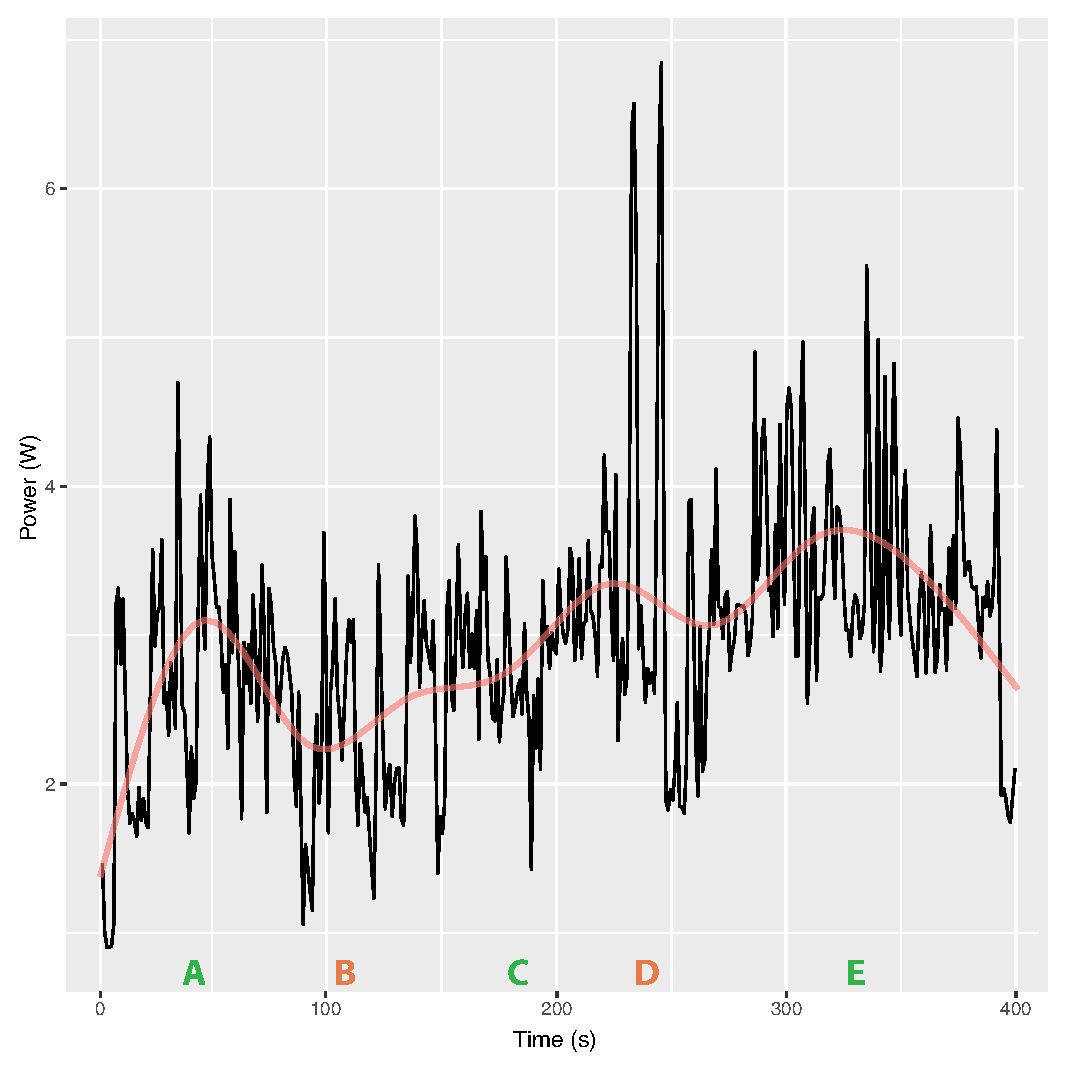
\includegraphics[width=0.5\linewidth]{figs/part_1_average_power}
    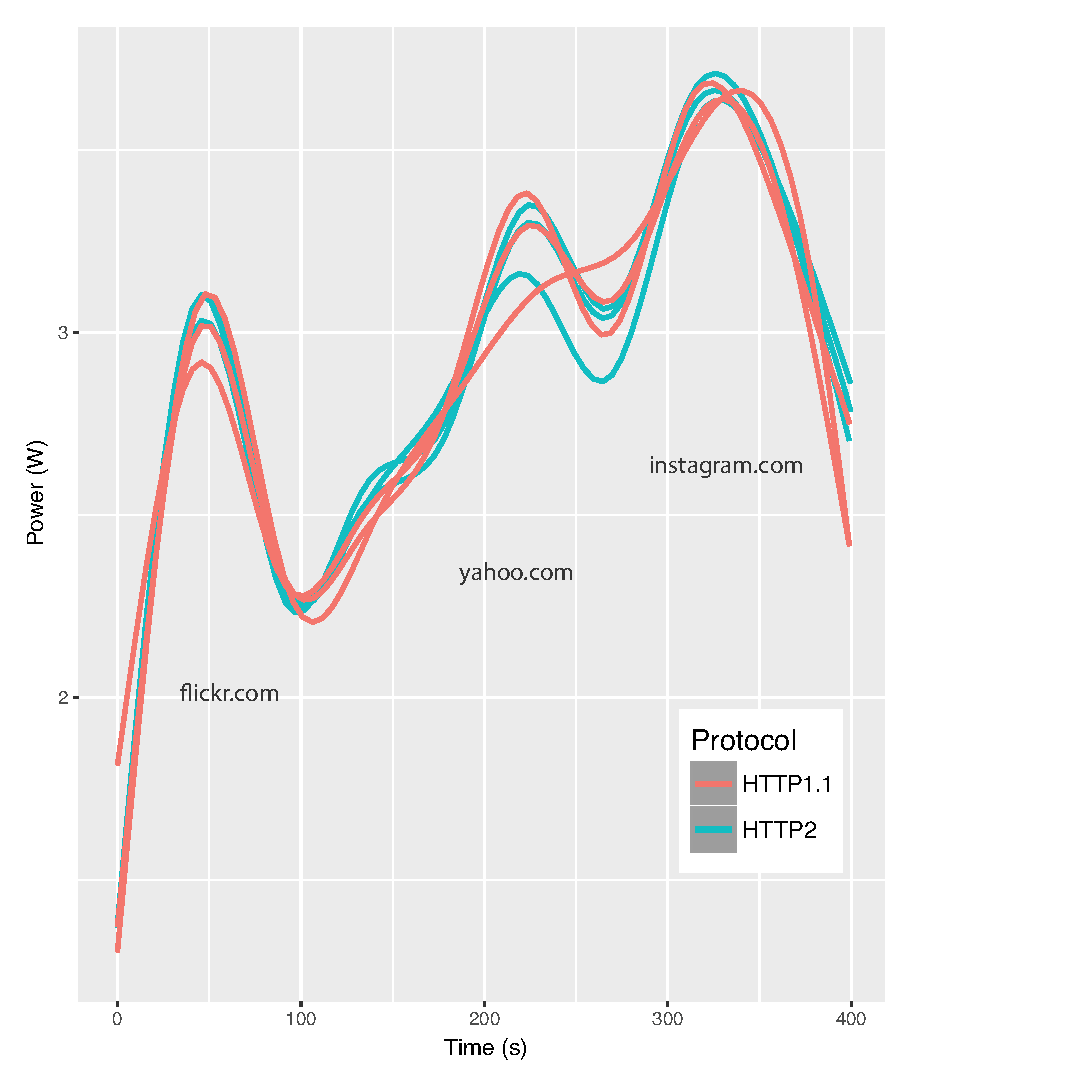
\includegraphics[width=0.5\linewidth]{figs/part_1_smoothed_power}
}
\begin{center}
    \textbf{Figure 1}: Average power draw of a test run done over HTTP1.1, and smoothed average of all six test runs done over HTTP1.1/HTTP2 during part I.
\end{center}
\vspace{-10mm}
\section{Results}

\textbf{Figure 1} and \textbf{Tables 1} and \textbf{2} present the energy consumption and network traffic statistics when browsing each of the three target websites over HTTP1.1 and HTTP2.2. Each line in \textbf{Figure 1} represents the average of 10 test runs done with a given combination of a target website, protocol and network condition. In \textbf{Tables 1} and \textbf{2} \emph{HL} refers to measurements done in high latency conditions ($\sim300$ms).

\columnbreak

\textbf{Table 1}: Energy consumption of the target websites over HTTP1.1 and HTTP2.

\begin{tabular}{|l|K{8cm}|K{8.1cm}|K{8cm}|}
    \hline
    \textcolor{blue}{HTTP1.1} / \textcolor{red}{HTTP2} & Total energy (J) & Power average (W) & Power std.dev (W) \\ \hline \hline
    Flickr & \textcolor{blue}{519.7} / \textcolor{red}{520.1}  &\textcolor{blue}{3.075} / \textcolor{red}{3.077}  & 
    \textcolor{blue}{0.832} / \textcolor{red}{0.748}  \\ \hline
    Flickr (HL) & \textcolor{blue}{659.8} / \textcolor{red}{532.3}  &\textcolor{blue}{3.315} / \textcolor{red}{3.149}  & 
    \textcolor{blue}{0.841} / \textcolor{red}{0.797}  \\ \hline \hline
    
    Instagram & \textcolor{blue}{631.4} / \textcolor{red}{646.2} & \textcolor{blue}{3.172} / \textcolor{red}{3.247} & \textcolor{blue}{0.705} / \textcolor{red}{0.754} \\ \hline
    
    Instagram (HL) & \textcolor{blue}{659.8} / \textcolor{red}{670.0} & \textcolor{blue}{3.315} / \textcolor{red}{3.366} & \textcolor{blue}{0.841} / \textcolor{red}{0.857} \\ \hline \hline
    
    Yahoo & \textcolor{blue}{417.4} / \textcolor{red}{413.9} &\textcolor{blue}{2.801} / \textcolor{red}{2.778}  & \textcolor{blue}{0.624} / \textcolor{red}{0.597}  \\ \hline 
    Yahoo (HL) & \textcolor{blue}{447.6} / \textcolor{red}{446.6} &\textcolor{blue}{3.004} / \textcolor{red}{2.997}  & \textcolor{blue}{0.586} / \textcolor{red}{0.611}  \\ \hline
\end{tabular}
\vspace{-2mm}
\begin{center}

\textbf{Table 2}: Network traffic statistics of each target website during the test runs.

\begin{tabular}{|l|K{7.2cm}|K{8cm}|K{7.5cm}|}
    \hline
    \textcolor{blue}{HTTP1.1} / \textcolor{red}{HTTP2} & Flickr & Instagram & Yahoo \\ \hline \hline
    Total Payload (kB) & \textcolor{blue}{63669} / \textcolor{red}{64853}  & \textcolor{blue}{33210} / \textcolor{red}{32664}  & 
    \textcolor{blue}{19833} / \textcolor{red}{20491}  \\ \hline
    Response Time (s) & \textcolor{blue}{1135} / \textcolor{red}{936}  &\textcolor{blue}{117} / \textcolor{red}{170}  & 
    \textcolor{blue}{127} / \textcolor{red}{119}  \\ \hline
    
    Number of Requests & \textcolor{blue}{587} / \textcolor{red}{606} & \textcolor{blue}{469} / \textcolor{red}{464} & \textcolor{blue}{511} / \textcolor{red}{509} \\ \hline \hline
    
    Total Bit Rate (kB/s) & \textcolor{blue}{56.1} / \textcolor{red}{69.3} & \textcolor{blue}{283.8} / \textcolor{red}{192.1} & \textcolor{blue}{156.2} / \textcolor{red}{172.2} \\  \hline
    
    Image Bit Rate (kB/s) & \textcolor{blue}{8.1} / \textcolor{red}{10.2} &\textcolor{blue}{51.9} / \textcolor{red}{33.2}  & \textcolor{blue}{18.8} / \textcolor{red}{24.4}  \\ \hline 
    
    JS Bit Rate (kB/s) & \textcolor{blue}{59.7} / \textcolor{red}{64.3} &\textcolor{blue}{354.5} / \textcolor{red}{301.8}  & \textcolor{blue}{87.2} / \textcolor{red}{87.8}  \\ \hline \hline
    
    Latency / RTT (ms) & $131.6\pm6.6$\newline(HL: $306\pm50.5$)	& $112.7\pm4.7$\newline(HL: $295.6\pm56.3$) & $133.3\pm8$\newline(HL: $304\pm77.8$)	\\ \hline
\end{tabular}
\end{center}
\vspace{8mm}
\centerline{
    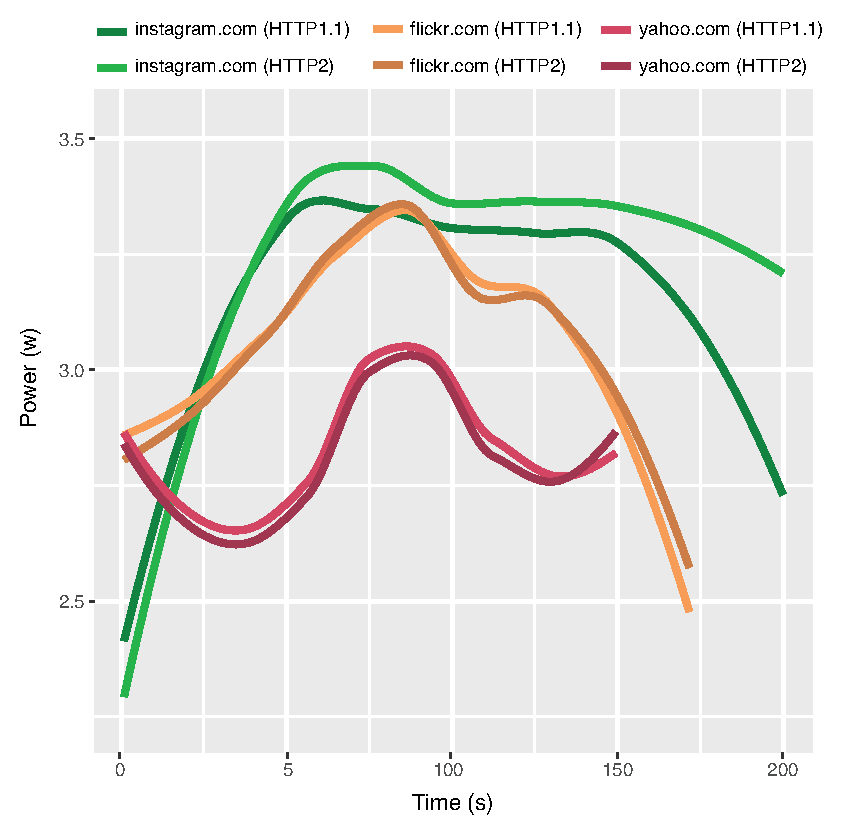
\includegraphics[width=0.5\linewidth]{figs/average}
    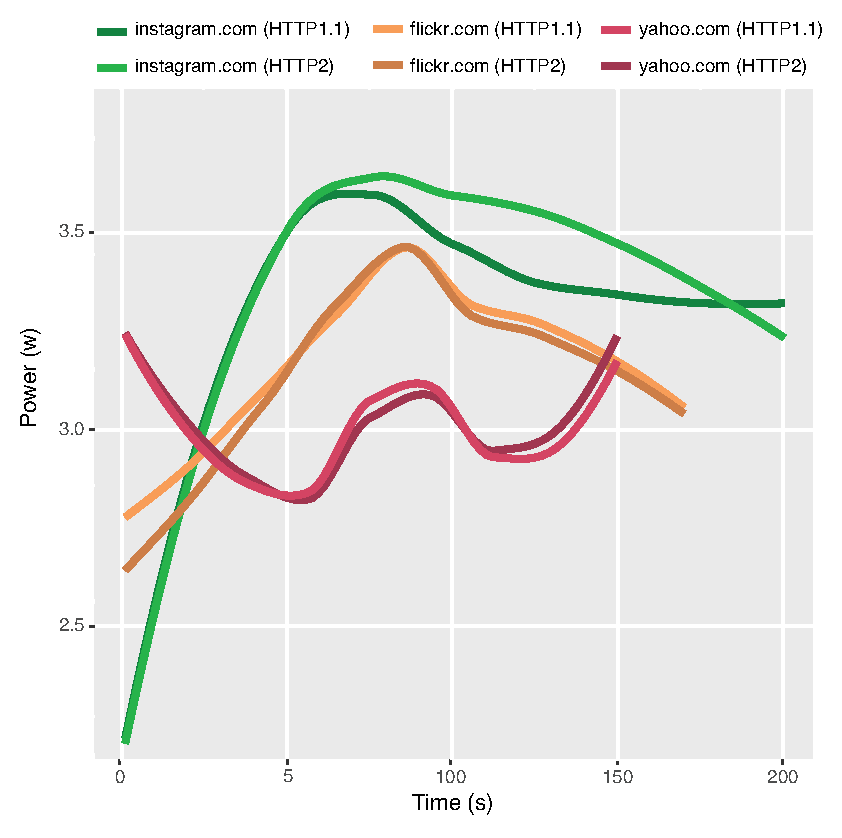
\includegraphics[width=0.5\linewidth]{figs/average-vpn}
}
\vspace{-6mm}
\begin{center}
    \textbf{Figure 2}: Power draw of browsing the target websites over HTTP1.1\newline and HTTP2 in low (left) and high (right) latency conditions.
\end{center}

\vspace{-13mm}
\section{Conclusions}
Only slight differences were observed between HTTP1.1 and HTTP2 energy consumption. Moreover, the better energy efficiency of HTTP2 fits within the error margin. As seen in \textbf{Table 2}, HTTP2 does however provide better energy utility (better bit rates with similar energy consumption). Though, this is not the case with Instagram, which exhibits longer response times and higher energy consumption over HTTP2. Observing the network waterfall of Instagram (omitted for brevity) it appears that image assets are stuck in \emph{Receiving} state longer and more often when requested over HTTP2. A more detailed explanation for this phenomenon will be provided in the final report.

\end{document}

